\PassOptionsToPackage{dvipsnames}{color}
\documentclass[10pt]{NSP1}
\usepackage{url,floatflt,cite}
\usepackage{helvet,times}
\usepackage{psfig,graphicx}
\usepackage{mathptmx,amsmath,amssymb,bm}
\usepackage{float}
\usepackage[bf,hypcap]{caption}
\usepackage{placeins}
\usepackage{booktabs}
\usepackage{array}
\usepackage{multirow}
\usepackage{makecell}
\graphicspath{{./images/}}

\definecolor{abstractcolor}{named}{Dandelion}
\definecolor{rulecolor}{named}{Bittersweet}

% Adjust margins
\addtolength{\oddsidemargin}{.5in}
\addtolength{\evensidemargin}{-.5in}

\tolerance=1
\emergencystretch=\maxdimen
\hyphenpenalty=10000
\hbadness=10000
\topmargin=0.00cm
\raggedbottom

\def\sm{\smallskip}
\def\no{\noindent}

\def\firstpage{185}
\setcounter{page}{\firstpage}
\def\thevol{10}
\def\thenumber{1}
\def\theyear{2026}

\begin{document}
	
	\titlefigurecaption{{
			\large \bf \rm Journal of Statistics Applications \& Probability
			\\
			\it\small An International Journal
	}}
	
	\title{A Hybrid Bellman--Ford--Dijkstra (DB) Algorithm for Efficient Shortest Path Computation}
	
	\author{Aijaz Ahmad Magray\hyperlink{author1}{$^{1}$}, D. Raju\hyperlink{author2}{$^{2}$}, Aafaq A. Rather\hyperlink{author3}{$^{3,*}$}, Ikram Ali\hyperlink{author4}{$^{4}$}, Vidya Yerneni\hyperlink{author5}{$^{3}$}, Ahmed A.F Osman\hyperlink{author6}{$^{5,*}$}, Mohammed Ataelfadiel\hyperlink{author7}{$^{5}$}, Ala Abdullah\hyperlink{author8}{$^{5}$}, Maryam Nasser Almusallam\hyperlink{author9}{$^{5}$}, Osman Elwasila Elshiekh\hyperlink{author10}{$^{6}$}, Ali Salem Bin Sama\hyperlink{author11}{$^{6}$} and P Srinivasa Rao\hyperlink{author12}{$^{7}$}}
	
	\institute{
		$^1$ Department of Mathematics, JB institute of engineering and technology, Hyderabad, 500075, India\\
		$^2$ Department of Mathematics, Jawaharlal Technological University, Kukatpally, Hyderabad - 500085, India\\
		$^{3}$ Symbiosis Statistical Institute, Symbiosis International (Deemed University), Pune, India\\
		$^4$ Assistant Professor Department of CSE, Apex Institute of Technology, Chandigarh University, Gharuan Mohali Punjab-412207, India\\
		$^{5}$ Applied College, King Faisal University, P.O. Box 400, Al-Ahsa 31982, Saudi Arabia\\
		$^{6}$ Department of Management Information Systems (MIS), College of Business Administration, King Faisal University, Al‑Ahsa, Eastern Province, Kingdom of Saudi Arabia\\
		$^{7}$ Department of Computer Science, JB institute of engineering and technology, Hyderabad, 500075, India
	}
	
	\titlerunning{A Hybrid Bellman--Ford--Dijkstra (DB) Algorithm...}
	\authorrunning{A. Magray et al.}
	
	\mail{aafaq7741@gmail.com, afadol@kfu.edu.sa}
	
	\received{-------}
	\revised{--------}
	\accepted{------}
	\published{1 ---. 20--}
	
	\abstracttext{In graph theory, detecting the shortest path between two active nodes remains a significant challenge in the research community. Finding the minimum-cost path between two nodes remains an important research problem with numerous practical applications. Although Dijkstra's algorithm provides efficient shortest-path computation for graphs with non-negative edge weights and Bellman-Ford handles negative edge weights, neither algorithm simultaneously offers efficient computation, reduced search space, and low computational overhead. This limitation motivates the development of a hybrid algorithm that combines the strengths of both approaches while overcoming their individual weaknesses. In this paper, we propose a novel hybrid DB Algorithm that integrates the Bellman--Ford and Dijkstra algorithms to efficiently compute shortest paths in weighted graphs containing negative edge weights while reducing computational time and search-space complexity. The proposed DB Algorithm addresses the limitations of existing shortest-path algorithms by reducing computational overhead while efficiently handling negative edge weights and minimizing time and space complexity. The proposed algorithm is evaluated using two key performance metrics: Time to search for the Shortest Distance (TSSD) and computational space complexity. Experimental results demonstrate that the proposed DB Algorithm significantly reduces computational overhead while accurately identifying shortest paths in weighted graphs. Simulation results validate the effectiveness and computational efficiency of the proposed DB Algorithm. In the future, the proposed DB Algorithm has potential applications to wireless communication systems, network routing, multidirectional communication protocols, and quantum computing applications.}
	
	\keywords{Hybrid, DB-Algorithm, Active Nodes, Shortest Distance (SD), Time to Search Shortest Distance}
	
	\maketitle
	
	\section{Introduction}
	
	The well-studied research topic in graph theory is the shortest-path. It is indeed a major issue and a serious challenge in the research community. The study of shortest path problems between the vertices (nodes) and edges (lines) in a graph is an active research topic for research community. Therefore, a great deal of attention has been paid in graph theory to optimizing shortest-path, with the minimum length criteria between two nodes. Therefore, numerous algorithms have been redesigned and implemented for finding a shortest path between two nodes. Due to its wide range of applications which include network routing protocols, route planning, traffic control, path finding in social networks, computer games, and transportation systems, forging us an exclusive state of shortest path issue in the graphs. The purpose to find the shortest path with all variants between two nodes in a graph is a complex act that needed to be resolved with the special techniques in mathematics. Several numbers of techniques suggested by the research scholars include Greedy algorithm, M. Fredman, Floyd Warshall algorithm \cite{Bellman1957,Bellman1958}, Dijkstra's shortest path algorithm \cite{Fredman1976,Floyd1962}, Bellman Ford-algorithm \cite{Warshall1962,Kim2022}, and Genetic algorithm for optimizing the route between the two nodes in a graph. These algorithms are designed to determine the shortest path in a graph. Shortest path algorithms constitute a family of algorithms used to solve shortest path problems.

	Several research solutions have been implemented to overcome the short path problems in a graph. However, they fail to address all the variant vulnerabilities of space and time that are associated with the shortest paths \cite{Coy2022,Gajjar2024}. Our aim is to present a new hybrid algorithm model which handles all inherited limitations and vulnerabilities that occur in previous algorithms. The new hybrid model has been proposed to sort out the time and space complexity issues for graph in this paper. It has an ability to find the shortest path between two vertices or nodes in graph theory.
	
	\section{The Proposed DB-Algorithm}
	
	The proposed DB-algorithm is the Hybridization of  two or more meta-heuristic optimization algorithms for searching for the most suitable and optimal solution in a specific search space \cite{Kim2025,Andreoletti2025}. The proposed DB-algorithm works on both positive and negative edge weights through parallel operations. Therefore, parallel operations of the proposed algorithm hold good properties which make it capable of working on different methods and resolving the problems efficiently. For example, searching is efficient when the problems can be solved with many solutions.

	Prime objective of Hybridization is as:
	\begin{enumerate}
		\item To address vulnerability of specific meta-heuristic optimization algorithm.
    
		\item To address limitations of specific meta-heuristic optimization algorithm.

		\item To counter disadvantages of specific meta-heuristic optimization algorithm.

		\item To integrate the advantages of specific meta-heuristic optimization algorithm.

    
	\end{enumerate}

	In the proposed DB Algorithm, Phase One (P1) represents a search-space pruning stage in which the Bellman--Ford algorithm is used to identify feasible shortest-path candidates while handling negative edge weights. This stage generates a reduced search space by eliminating infeasible or non-promising paths. Phase Two (P2) applies Dijkstra's algorithm to the reduced search space generated in Phase One, thereby improving computational efficiency. Therefore, the term ``phase'' refers to two sequential computational stages rather than graph clustering, and no partitioning of vertices into mathematical clusters is performed. Figure~\ref{fig:hybridization} depicts the concept of hybridization of two meta-heuristic optimization algorithms which addresses the limitations and vulnerabilities by integrating the advantages of other meta-heuristic optimization algorithm and facilitates commitment for convergence with fewer time parameters and space complexity.
    
\setlength{\floatsep}{6pt}   
\setlength{\textfloatsep}{6pt}  
\setlength{\intextsep}{6pt} 

\begin{figure}[!b]
    \centering
    
    \begin{minipage}{0.48\textwidth}
        \centering
        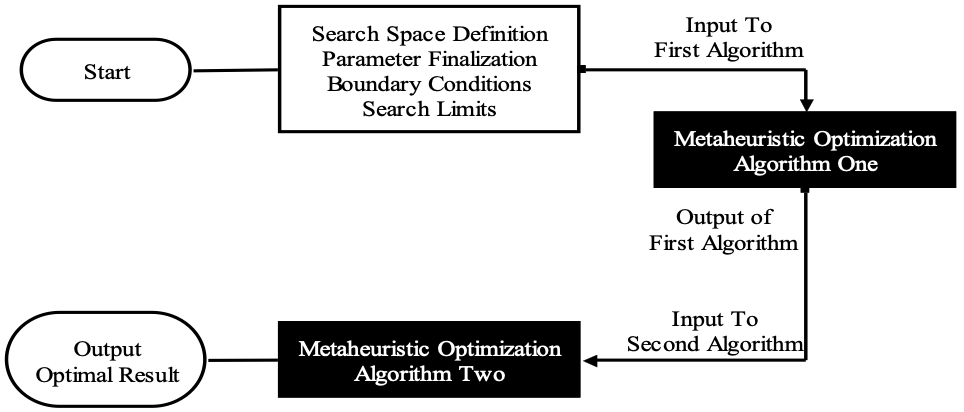
\includegraphics[width=8cm, height=6cm]{fig1.png}
        \caption{Hybridization of Two Optimization Algorithm}
        \label{fig:hybridization}
    \end{minipage}
    \hfill
    \begin{minipage}{0.48\textwidth}
        \centering
        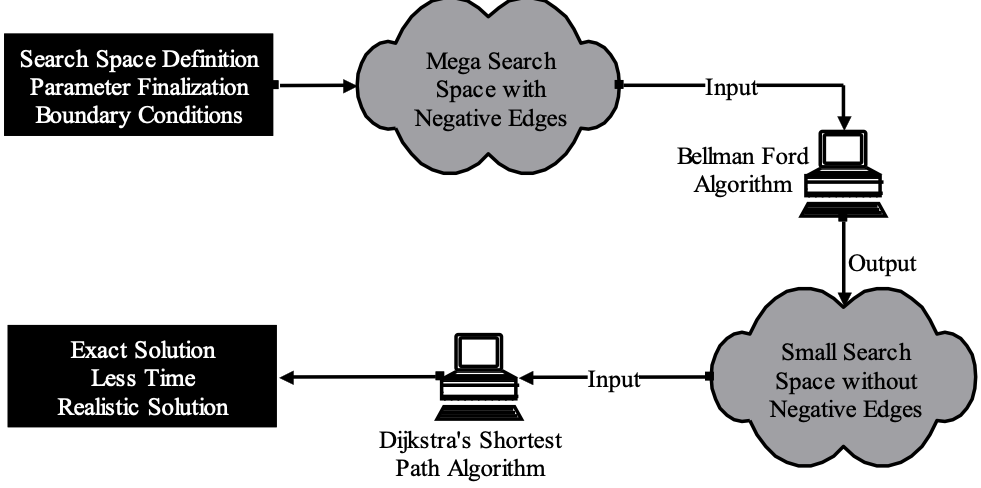
\includegraphics[width=8cm, height=6cm]{fig2.png}
        \caption{The proposed DB-Algorithm}
        \label{fig:proposed_db}
    \end{minipage}
\end{figure}

~

	Hence, the proposed DB-Algorithm is a possible method for solving the negative weights in the search space. It can overcome the limitations which are constituted by the previous designs. The proposed algorithm can perform parallel search of various nodes in space which has the ability to consume less time in space to achieve target. This ability will become a benchmark to be the fastest algorithm. Dijkstra's shortest path algorithm has a blind search. It calculates the entire path from source to destination, which makes algorithm inefficient because it wastes more time to reach to the necessary-resources. In addition, if the space search of an algorithm increases, the time required for the optimal path also increases exponentially. In addition, it works with non-negative weights for the edges with slight modifications but fails for negative weight in the space graph, which swings the system and hangs the final results. However, nested loops taken by Dijkstra's algorithm leads to increase the search time in space \cite{Hlupic2025,Dory2025}. Due to some limitations of Dijkstra's algorithm like using nested loops, which increase the search time, it becomes necessary work for research community to implement a new algorithm which can span less time in space, using limited loops. In this regard a new DB-Algorithm algorithm has been proposed.

~

	The proposed DB-algorithm provides a more accurate and realistic approach in nature in the context of real-world problems. The DB-algorithm works with both positive and negative edge weights. It overcomes the limitations of Dijkstra's Algorithm. Initially Bellman-Ford-algorithm is initiated with parameter subjected to target search space; the output of this search will be input for Dijkstra's Algorithm and is search space for the second algorithm. However, the proposed algorithm is shown in Figure~\ref{fig:proposed_db}, which is free of negative edges and is smaller in size than previous designs.

	
	
\section{The Java Code Segment using for the proposed DB-Algorithm}
	
	Optimal Shortest Path selection process for the proposed DB-algorithm has been checked in the java cod as:
	\begin{center}
	\begin{minipage}{0.52\columnwidth}
	\small
	\begin{tabbing}
		\quad \= \quad \= \quad \= \quad \= \quad \= \kill
		\textbf{Declare} $\text{Int}\ N\_D\ \text{Number\_of\_Node},\ N\_C\ \text{Number\_of\_Cluster},\ D\_N\ \text{Distance Between Nodes}$ \\
		$\text{Int}\ {N_L}\ \text{Loop\_1\_Count},\ {N_{L2}} \ \text{Loop\_2\_Count}$ \\[5pt]
		\textbf{Start phase one - Level 1} \\
		\> \textbf{Start phase one - Level 2} \\
		\> \> \textbf{Start phase one - Level 3} \\
		\> \> \> \textbf{Repeat-Step-3 for} $i = 1, 2, \dots, n$ \textbf{Start-Loop One} \\
		\> \> \> \> \textbf{Repeat-loop for} $i = 1, 2, \dots, n$ \textbf{Start-Loop Two} \\
		\> \> \> \> \> Optimal Cluster Selection Process Start \\
		\> \> \> \> \> Check if $a[V_s, i] = 0$ \\
		\> \> \> \> \> Optimal Shortest Path Selection Process Start \\
		\> \> \> \> \> In case no direct-edge among $V_s$ \& $V_i$ \\
		\> \> \> \> \> \textbf{Then:} $\text{leng}[i] = \text{Infinity}$ [Infinity value is taken to be 999] \\
		\> \> \> \> \> \phantom{\textbf{Then:}} $\text{path}[i] = 0$ [Invalid path] \\
		\> \> \> \> \> \textbf{Else:} $\text{leng}[i] = a[V_s, i]$ and $\text{path}[i] = V_s$ \\
		\> \> \textbf{End Phase One - Level\_3} \\
		\> \textbf{End Phase\_One - Level\_2} \\
		\textbf{End Phase\_One Level - 1} \\[8pt]
		\textbf{Second Level Clustering Start with new non negative search space, shortened search space} \\
		\textbf{Start Phase Two Level\_1} \\
		\> \textbf{Start Phase Two Level\_2} \\
		\> \> \textbf{Start Phase Two Level\_3} \\
		\> \> \> \textbf{Repeat-Step3-for} $i = 1, 2, \dots, n$ \textbf{Start Loop One} \\
		\> \> \> \> \textbf{Repeat-loop for} $i = 1, 2, \dots, n$ \textbf{Start Loop Two} \\
		\> \> \> \> \> Optimal Cluster Selection Process Start \\
		\> \> \> \> \> Check if $a[V_s, i] = 0$ \\
		\> \> \> \> \> Optimal Shortest Path Selection Process Start \\
		\> \> \> \> \> In case no-direct edge among $V_s$ \& $V_i$ \\
		\> \> \> \> \> \textbf{Then:} $\text{leng}[i] = \text{Infinity}$ [Infinity-value is taken to-be 999] \\
		\> \> \> \> \> \phantom{\textbf{Then:}} $\text{path}[i] = 0$ [Invalid path] \\
		\> \> \> \> \> \textbf{Else:} $\text{leng}[i] = a[V_s, i]$ and $\text{path}[i] = V_s$ \\
		\> \> \textbf{End Phase\_Two Level\_3} \\
		\> \textbf{End Phase\_Two Level\_2} \\
		\textbf{End Phase\_Two Level\_1} \\[5pt]
		\textbf{Optimal Shortest Path Selection Process End: Print Result.}
	\end{tabbing}
	\end{minipage}
	\end{center}
	
	
\section{Flow Chart}
	
	Figure~\ref{fig:flowchart} describes the flow chart of the proposed algorithm.
	
	\begin{figure}[H]
		\centering
		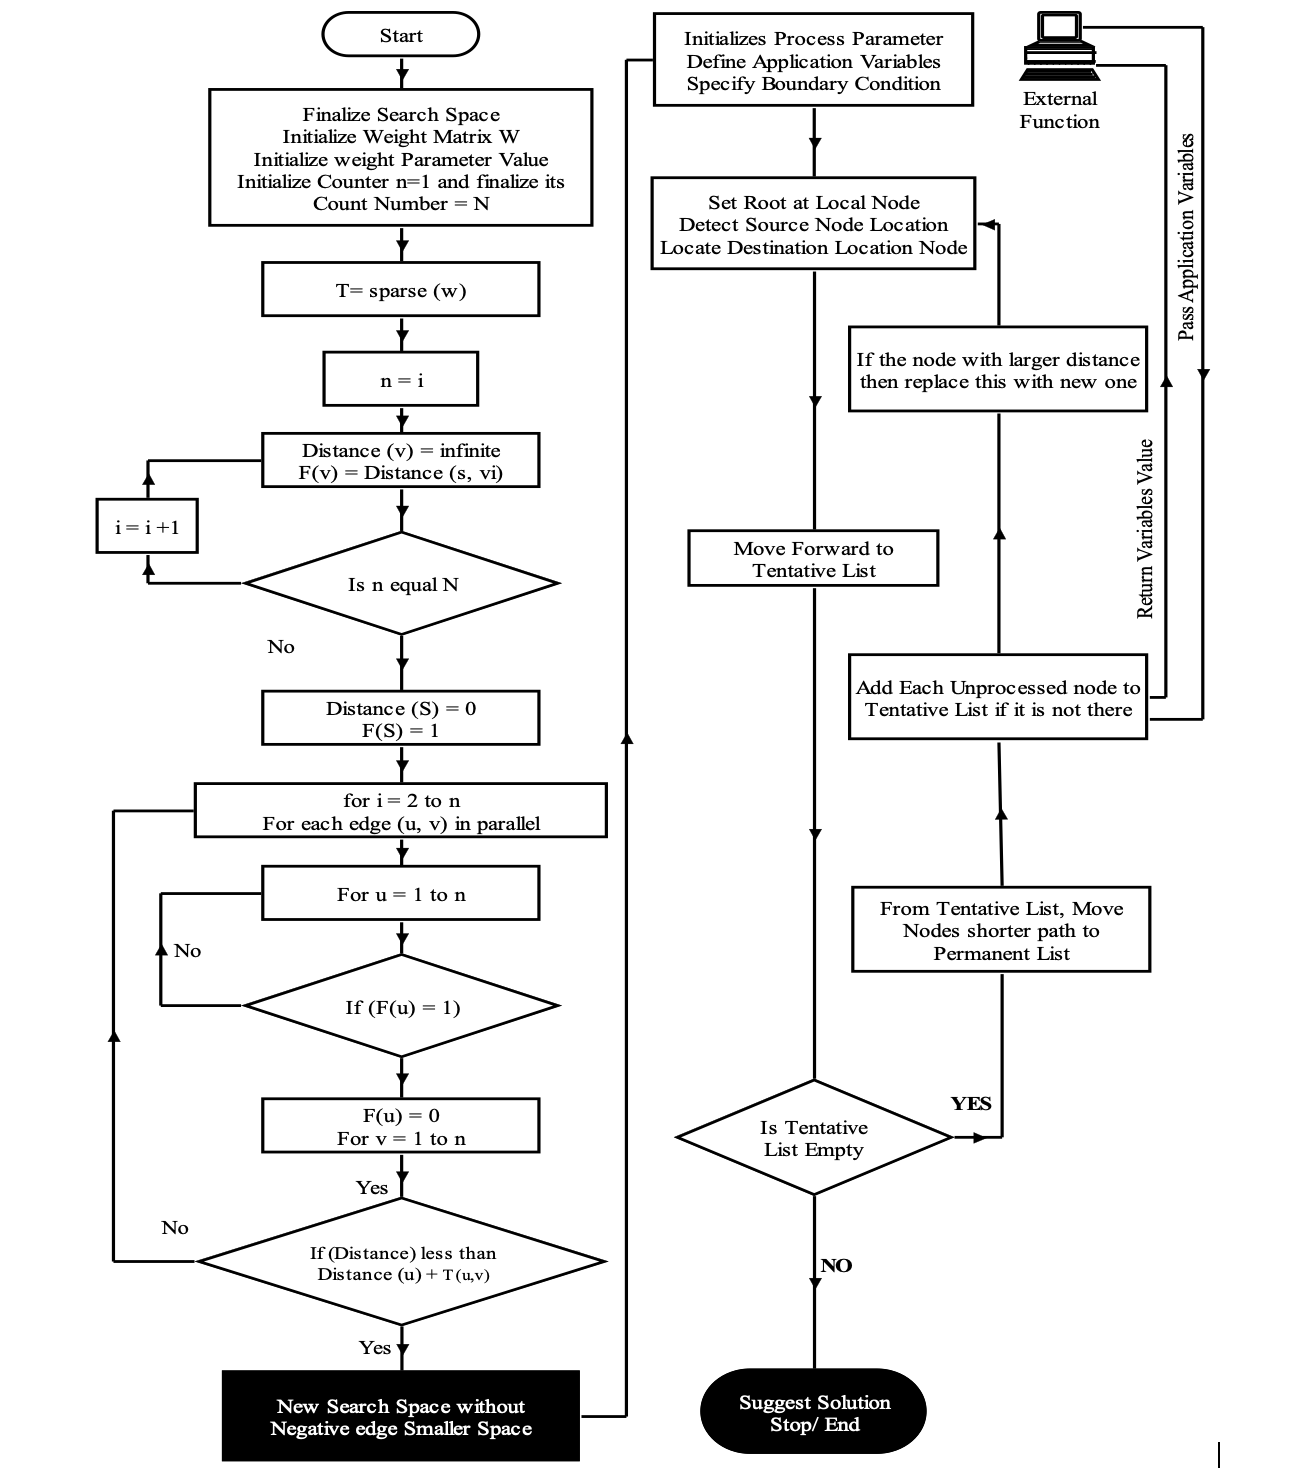
\includegraphics[width=12cm, height=17cm]{fig3.png}
		\caption{The Proposed DB-Algorithm Flow Chart}
		\label{fig:flowchart}
	\end{figure}
	
	\section{Result}
	
	\subsection{System Configuration}
	\begin{itemize}
		\item \textbf{Machine:} Dell Latitude 3440
		\item \textbf{Processor:} 13th Gen Intel\textregistered\ Core\texttrademark\ i7-1355U, 1.70 GHz
		\item \textbf{RAM:} 16.0 GB (15.7 GB usable)
		\item \textbf{Operating System:} Windows 11 Education, Version 23H2 (OS Build 22631.4391)
		\item \textbf{System Type:} 64-bit operating system, x64-based processor
		\item \textbf{Device ID:} C7C2F718-4A80-4576-94C2-E6A7EEF45FCA
		\item \textbf{Windows Feature Experience Pack:} 1000.22700.1047.0
	\end{itemize}
	
\subsection{Graphs with 3 vertices}
	
	We tested the algorithms with graphs containing 0, 1 and 2 vertices, using different paths. The execution time of the DB algorithm was calculated and compared with that of Dijkstra's algorithm. All the test results are provided below (see Figure~\ref{fig:graph3} for a graphical representation and Table~\ref{tab:adj3} for detailed numerical values), and the result is clearly mentioned in Table~\ref{tab:results3}.
	
	\begin{figure}[H]
			\centering
			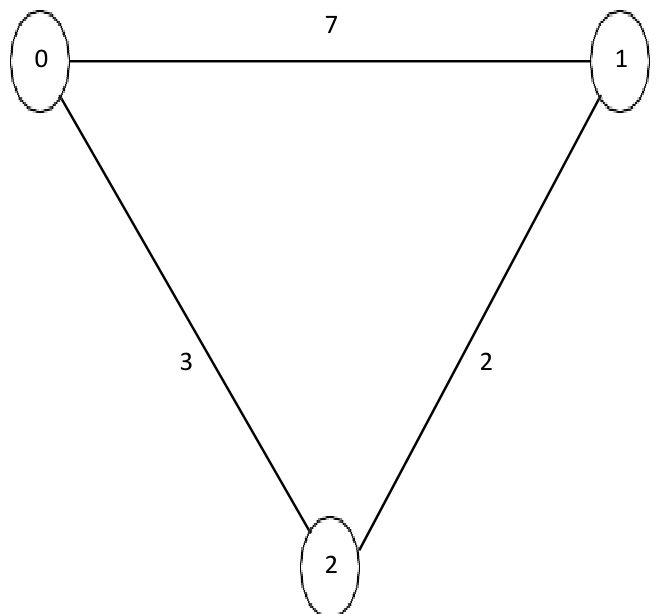
\includegraphics[width=0.3\linewidth]{fig4.png}
			\caption{Graph with Shortest path}
			\label{fig:graph3}
\end{figure}

\begin{table}[H]
			\centering
			\captionof{table}{Adjacency Matrix of 3 vertices}
			\label{tab:adj3}
			\vspace{5pt}
			% أوامر التكبير
			\Large
			\setlength{\tabcolsep}{12pt}   % تباعد أفقي كبير بين الخلايا
			\renewcommand{\arraystretch}{1.5} % تباعد رأسي مريح
			\begin{tabular}{|c|c|c|c|}
				\hline
				& \textbf{0} & \textbf{1} & \textbf{2} \\
				\hline
				\textbf{0} & 0 & 7 & 3 \\
				\hline
				\textbf{1} & 7 & 0 & 2 \\
				\hline
				\textbf{2} & 3 & 2 & 0 \\
				\hline
			\end{tabular}
\end{table}
	
	\begin{table}[H]
		\centering
		\caption{Shortest path and execution time table (3 vertices)}
		\label{tab:results3}
		\vspace{5pt}
		
		\small
		\setlength{\tabcolsep}{5pt}
		\renewcommand{\arraystretch}{1.4}
		\begin{tabular}{|c|c|c|c|c|c|c|c|}
			\hline
			\multirow{2}{*}{\textbf{Sr. No.}} & \multirow{2}{*}{\textbf{Vertex}} & \textbf{Target} & \textbf{Possible Best} & \textbf{Total} & \textbf{Dijkstra Algorithms} & \multicolumn{2}{c|}{\textbf{DB Algorithms}} \\
			\cline{7-8}
			& & \textbf{\makecell{Target\\(Source-to-Dest.)}} & \textbf{\makecell{Possible Best\\Shortest Path}} & \textbf{\makecell{Total\\Distance}} & \textbf{\makecell{Execution Time\\Complexity}} & \textbf{\makecell{Execution Time\\Complexity}} & \textbf{\makecell{Convert to\\(Nano Second)}} \\
			\hline
			01 & 03 & 0--1 & 0--2--1 & 5 & 19779800 ns & 0.1005 ms & 100,500 ns \\
			\hline
			02 & 03 & 1--0 & 1--2--0 & 5 & 18160900 ns & 0.083 ms & 83,000 ns \\
			\hline
			03 & 03 & 2--1 & 2--1 & 2 & 19289700 ns & 0.0873 ms & 87,300 ns \\
			\hline
			04 & 03 & 2--0 & 2--0 & 3 & 19910900 ns & 0.0924 ms & 92,400 ns \\
			\hline
			\multicolumn{5}{|c|}{\textbf{Average Execution Time}} & \textbf{19285325 ns} & -- & \textbf{363200 ns} \\
			\hline
		\end{tabular}
	\end{table}
	
	Execution time calculated based on different shortest paths:
	\begin{align}
		\text{Percentage Faster} &= \frac{\text{Dijkstra Algorithms Average} - \text{DB Algorithms Average}}{\text{Dijkstra Algorithms Average}} \times 100 \notag \\
		&= \frac{19285325 - 363200}{19285325} \times 100 \notag \\
		&= \frac{18922125}{19285325} \times 100 \notag \\
		&= 98.12\%
	\end{align}
	
	Figure~\ref{fig:graph3} and Table~\ref{tab:results3} demonstrate the performance of the proposed DB Algorithm on a small graph containing three vertices. The algorithm correctly identifies the shortest paths while reducing the search space before applying Dijkstra's algorithm. The experimental results show that the hybrid approach significantly decreases execution time without affecting the correctness of the computed shortest paths.

\subsection{Graph with vertex -4}
	
	We tested the algorithms with graphs containing 4 vertices shown in Figure~\ref{fig:graph4} using different paths. The execution time of the DB algorithm was calculated and compared with that of Dijkstra's algorithm. All the test results are provided and mentioned in Table~\ref{tab:adj4} and Table~\ref{tab:results4} determines the shortest path and execution time which clearly shows that DB algorithm result is 99.50\% better than Dijkstra's algorithm.
    
	\begin{figure}[H]
			\centering
			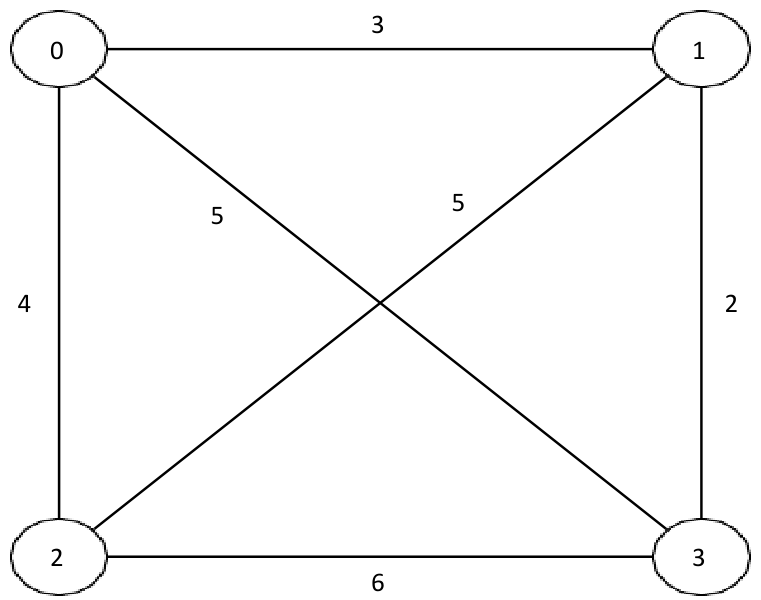
\includegraphics[width=0.4\linewidth]{fig5.png}
			\caption{Graph with shortest path}
			\label{fig:graph4}
\end{figure}

\begin{table}[H]
			\centering
			\captionof{table}{Adjacency Matrix of 4 vertices}
			\label{tab:adj4}
			\vspace{5pt}
			% أوامر تكبير الجدول
			\Large
			\setlength{\tabcolsep}{14pt}   % تباعد أفقي أكبر بين الخلايا
			\renewcommand{\arraystretch}{1.6} % تباعد رأسي أكبر بين الصفوف
			\begin{tabular}{|c|c|c|c|c|}
				\hline
				& \textbf{0} & \textbf{1} & \textbf{2} & \textbf{3} \\
				\hline
				\textbf{0} & 0 & 3 & 4 & 5 \\
				\hline
				\textbf{1} & 3 & 0 & 5 & 2 \\
				\hline
				\textbf{2} & 4 & 5 & 0 & 6 \\
				\hline
				\textbf{3} & 5 & 2 & 6 & 0 \\
				\hline
			\end{tabular}
	\end{table}
	
	\begin{table}[H]
		\centering
		\caption{Shortest path and execution time table (4 vertices)}
		\label{tab:results4}
		\vspace{5pt}
		\setlength{\tabcolsep}{2.5pt}
		\begin{tabular}{|c|c|c|c|c|c|c|c|}
			\hline
			\multirow{2}{*}{\textbf{Sr. No.}} & \multirow{2}{*}{\textbf{Vertex}} & \textbf{Target} & \textbf{Possible Best} & \textbf{Total} & \textbf{Dijkstra Algorithms} & \multicolumn{2}{c|}{\textbf{DB Algorithms}} \\
			\cline{7-8}
			& & \textbf{\makecell{Target\\(Source-to-Dest.)}} & \textbf{\makecell{Possible Best\\Shortest Path}} & \textbf{\makecell{Total\\Distance}} & \textbf{\makecell{Execution Time\\Complexity}} & \textbf{\makecell{Execution Time\\Complexity}} & \textbf{\makecell{Convert to\\(Nano Second)}} \\
			\hline
			01 & 4 & 1--2 & 1--2 & 5 & 27752100 ns & 0.0889 ms & 88900 ns \\
			\hline
			02 & 4 & 0--3 & 0--1--3 & 5 & 21884000 ns & 0.122 ms & 122000 ns \\
			\hline
			03 & 4 & 3--0 & 3--0 & 5 & 20483600 ns & 0.125 ms & 125000 ns \\
			\hline
			04 & 4 & 2--3 & 2--3 & 6 & 23297200 ns & 0.098 ms & 98000 ns \\
			\hline
			05 & 4 & 2--0 & 2--0 & 4 & 17697000 ns & 0.1159 ms & 115900 ns \\
			\hline
			\multicolumn{5}{|c|}{\textbf{Average Execution Time}} & \textbf{22222780 ns} & -- & \textbf{109960 ns} \\
			\hline
		\end{tabular}
	\end{table}
	
	Execution Time Calculated based on different shortest paths:
	\begin{align}
		\text{Percentage Faster} &= \frac{\text{Dijkstra's Algorithms Average} - \text{DB Algorithms Average}}{\text{Dijkstra's Algorithms Average}} \times 100 \notag \\
		&= \frac{22222780 - 109960}{22222780} \times 100 \notag \\
		&= \frac{22112820}{22222780} \times 100 \notag \\
		&\cong 99.50\%
	\end{align}
	
	Figure~\ref{fig:graph4} and Table~\ref{tab:results4} evaluate the proposed algorithm on a graph with four vertices. As the graph size increases, the DB Algorithm maintains accurate shortest-path computation while efficiently handling the reduced search space generated during Phase One. The results indicate that the computational advantage is preserved as graph complexity increases.
    
\setlength{\floatsep}{2pt}      % Space between floats
\setlength{\textfloatsep}{2pt}  % Space between float and text
\setlength{\intextsep}{2pt} 

\subsection{Graph with vertex -6}
	
	The third test was on the 6 vertices with so many shortest paths between source to destination as shown in Figure~\ref{fig:graph6} and also in Table~\ref{tab:adj6} determines the weight and paths. The execution time mentioned in Table~\ref{tab:results6} was calculated and compared with Dijkstra's algorithm, which shows 96.23\% better result than the available algorithm.
	
	\begin{figure}[H]
			\centering
			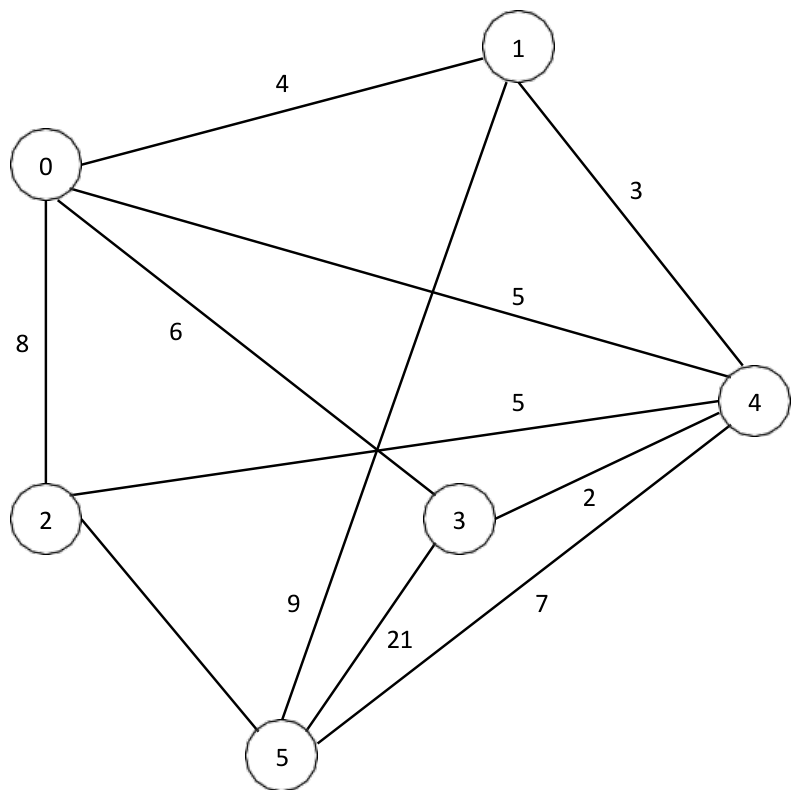
\includegraphics[width=0.6\linewidth]{fig6.png}
			\caption{Graph with Shortest Path}
			\label{fig:graph6}
\end{figure}

\begin{table}[H]
			\centering
			\captionof{table}{Adjacency Matrix of 6 vertices}
			\label{tab:adj6}
			\setlength{\tabcolsep}{3pt}
			\begin{tabular}{|c|c|c|c|c|c|c|}
				\hline
				\textbf{Vertex} & \textbf{0} & \textbf{1} & \textbf{2} & \textbf{3} & \textbf{4} & \textbf{5} \\
				\hline
				\textbf{0} & 0 & 4 & 8 & 6 & 5 & 0 \\
				\hline
				\textbf{1} & 4 & 0 & 0 & 0 & 3 & 9 \\
				\hline
				\textbf{2} & 8 & 0 & 0 & 0 & 5 & 6 \\
				\hline
				\textbf{3} & 6 & 0 & 0 & 0 & 2 & 4 \\
				\hline
				\textbf{4} & 5 & 3 & 5 & 2 & 0 & 7 \\
				\hline
				\textbf{5} & 0 & 9 & 6 & 4 & 7 & 0 \\
				\hline
			\end{tabular}
	\end{table}
	
	\begin{table}[H]
		\centering
		\caption{Shortest path and execution timetable (6 vertices)}
		\label{tab:results6}
		\setlength{\tabcolsep}{2.5pt}
		\begin{tabular}{|c|c|c|c|c|c|c|c|}
			\hline
			\multirow{2}{*}{\textbf{Sr. No.}} & \multirow{2}{*}{\textbf{Vertex}} & \textbf{Target} & \textbf{Possible Best} & \textbf{Total} & \textbf{Dijkstra Algorithms} & \multicolumn{2}{c|}{\textbf{DB Algorithms}} \\
			\cline{7-8}
			& & \textbf{\makecell{Target\\(Source-to-Dest.)}} & \textbf{\makecell{Possible Best\\Shortest Path}} & \textbf{\makecell{Total\\Distance}} & \textbf{\makecell{Execution Time\\Complexity}} & \textbf{\makecell{Execution Time\\Complexity}} & \textbf{\makecell{Convert to\\(Nano Second)}} \\
			\hline
			01 & 6 & 0--5 & 0--3--5 & 10 & 15983400 ns & 0.1304 ms & 130400 ns \\
			\hline
			02 & 6 & 3--2 & 3--4--2 & 7 & 16126100 ns & 0.1332 ms & 133200 ns \\
			\hline
			03 & 6 & 1--3 & 1--4--3 & 5 & 15518600 ns & 0.1343 ms & 134300 ns \\
			\hline
			04 & 6 & 2--1 & 2--4--1 & 8 & 15083500 ns & 0.1246 ms & 124600 ns \\
			\hline
			05 & 6 & 4--0 & 4--0 & 5 & 21313100 ns & 0.1094 ms & 109400 ns \\
			\hline
			\multicolumn{5}{|c|}{\textbf{Average Execution Time}} & \textbf{16804940 ns} & -- & \textbf{631900 ns} \\
			\hline
		\end{tabular}
	\end{table}
	
	Execution Time Calculated based on different shortest paths:
	\begin{align}
		\text{Percentage Faster} &= \frac{\text{Dijkstra Algorithms Average} - \text{DB Algorithms Average}}{\text{Dijkstra Algorithms Average}} \times 100 \notag \\
		&= \frac{16804940 - 631900}{16804940} \times 100 \notag \\
		&= \frac{16173040}{16804940} \times 100 \notag \\
		&= 96.23\%
	\end{align}
	
	Figure~\ref{fig:graph6} and Table~\ref{tab:results6} illustrate the behavior of the proposed algorithm on a denser graph with six vertices and multiple candidate paths. The reduced search space enables the algorithm to avoid unnecessary computations, resulting in consistent execution-time improvements while maintaining optimal path selection.

	\subsection{Graph with vertex -10}
	
	Finally, the testing was done on the 10 vertices shown in Figure~\ref{fig:graph10} and so many shortest paths were available from source to destination mentioned in Table~\ref{tab:adj10} and the execution time for the determination of shortest path was calculated which shows 98.91\% better result than the Dijkstra's algorithm which is mentioned in Table~\ref{tab:results10}.
    

	\begin{figure}[H]
			\centering
			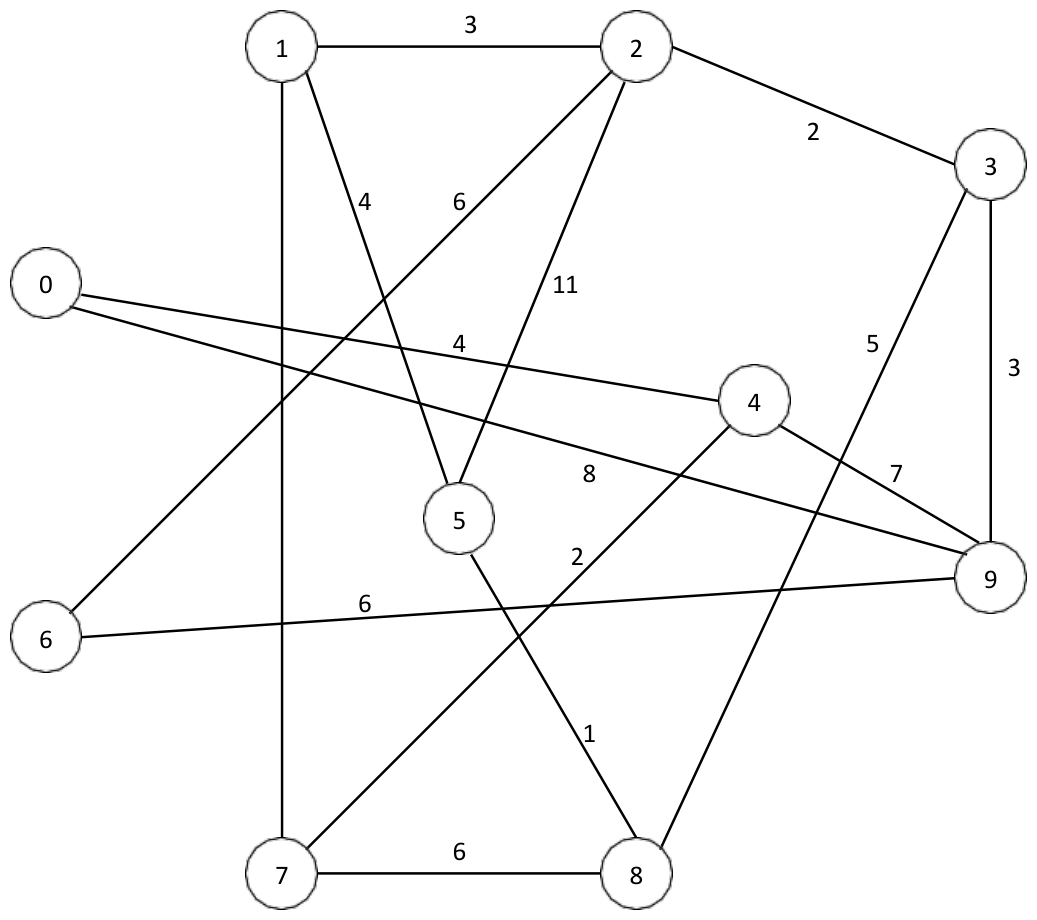
\includegraphics[width=0.6\linewidth]{fig7.png}
			\caption{Graph with Shortest path}
			\label{fig:graph10}
\end{figure}

\begin{table}[H]
			\centering
			\captionof{table}{Adjacency Matrix of 10 vertices}
			\label{tab:adj10}
			\vspace{5pt}
			\setlength{\tabcolsep}{1.8pt}
			\begin{tabular}{|c|c|c|c|c|c|c|c|c|c|c|}
				\hline
				\textbf{Vertex} & \textbf{0} & \textbf{1} & \textbf{2} & \textbf{3} & \textbf{4} & \textbf{5} & \textbf{6} & \textbf{7} & \textbf{8} & \textbf{9} \\
				\hline
				\textbf{0} & 0 & 0 & 0 & 0 & 7 & 0 & 0 & 0 & 0 & 8 \\
				\hline
				\textbf{1} & 0 & 0 & 3 & 0 & 0 & 4 & 0 & 7 & 0 & 0 \\
				\hline
				\textbf{2} & 0 & 3 & 0 & 2 & 0 & 11 & 6 & 0 & 0 & 0 \\
				\hline
				\textbf{3} & 0 & 0 & 2 & 0 & 0 & 0 & 0 & 0 & 5 & 3 \\
				\hline
				\textbf{4} & 7 & 0 & 0 & 0 & 0 & 0 & 0 & 2 & 0 & 7 \\
				\hline
				\textbf{5} & 0 & 4 & 11 & 0 & 0 & 0 & 0 & 0 & 1 & 0 \\
				\hline
				\textbf{6} & 0 & 0 & 6 & 0 & 0 & 0 & 0 & 0 & 0 & 6 \\
				\hline
				\textbf{7} & 0 & 4 & 0 & 0 & 2 & 0 & 0 & 0 & 6 & 0 \\
				\hline
				\textbf{8} & 0 & 0 & 0 & 5 & 0 & 1 & 0 & 6 & 0 & 0 \\
				\hline
				\textbf{9} & 8 & 0 & 0 & 3 & 7 & 0 & 6 & 0 & 0 & 0 \\
				\hline
			\end{tabular}
	\end{table}
	
	\begin{table}[H]
		\centering
		\caption{Shortest path and execution timetable (10 vertices)}
		\label{tab:results10}
		\vspace{5pt}
		\setlength{\tabcolsep}{2.5pt}
		\begin{tabular}{|c|c|c|c|c|c|c|c|}
			\hline
			\multirow{2}{*}{\textbf{Sr. No.}} & \multirow{2}{*}{\textbf{Vertex}} & \textbf{Target} & \textbf{Possible Best} & \textbf{Total} & \textbf{Dijkstra Algorithms} & \multicolumn{2}{c|}{\textbf{DB Algorithms}} \\
			\cline{7-8}
			& & \textbf{\makecell{Target\\(Source-to-Dest.)}} & \textbf{\makecell{Possible Best\\Shortest Path}} & \textbf{\makecell{Total\\Distance}} & \textbf{\makecell{Execution Time\\Complexity}} & \textbf{\makecell{Execution Time\\Complexity}} & \textbf{\makecell{Convert to\\(Nano Second)}} \\
			\hline
			01 & 10 & 0--8 & 0--4--7--8 & 15 & 16122500 ns & 0.2489 ms & 248900 ns \\
			\hline
			02 & 10 & 2--7 & 2--1--7 & 10 & 17276000 ns & 0.1233 ms & 123300 ns \\
			\hline
			03 & 10 & 3--5 & 3--8--5 & 6 & 17898500 ns & 0.153 ms & 153000 ns \\
			\hline
			04 & 10 & 1--9 & 1--2--3--9 & 8 & 16636500 ns & 0.1364 ms & 136400 ns \\
			\hline
			05 & 10 & 4--6 & 4--9--6 & 13 & 15989900 ns & 0.2502 ms & 250200 ns \\
			\hline
			\multicolumn{5}{|c|}{\textbf{Average Execution Time}} & \textbf{16784680 ns} & -- & \textbf{182360 ns} \\
			\hline
		\end{tabular}
	\end{table}
	
	Execution Time Calculated based on different shortest paths:
	\begin{align}
		\text{Percentage Faster} &= \frac{\text{Dijkstra Algorithms Average} - \text{DB Algorithms Average}}{\text{Dijkstra Algorithms Average}} \times 100 \notag \\
		&= \frac{16784680 - 182360}{16784680} \times 100 \notag \\
		&= \frac{16602320}{16784680} \times 100 \notag \\
		&\cong 98.91\%
	\end{align}
	
	Figure~\ref{fig:graph10} and Table~\ref{tab:results10} demonstrate the scalability of the proposed DB Algorithm on a larger graph consisting of ten vertices. Despite the increased number of possible routes, the hybrid approach continues to identify optimal shortest paths efficiently. These results indicate that the proposed method scales well with increasing graph size while maintaining computational efficiency.

\section{The DB -Algorithm facilitates various advantages like}
	
	\begin{itemize}\setlength{\itemsep}{2pt}\setlength{\parskip}{0pt}
		\item[\textbf{a)}] Negative weight or edge present in the search space is a major issue in Dijkstra's algorithms which has been countered in initial stage in DB-Algorithm such that new search space is suggested for optimal result.
		\item[\textbf{b)}] Dijkstra's algorithm implements recursive search technique which calls another function for optimization, this recursive calling results increases search time However, in the proposed DB-Algorithm already shortened the search space, now Dijkstra's algorithm required confining the search in smaller space, this technique saves time and resources.
		\item[\textbf{c)}] The proposed DB Algorithm significantly reduces the possibility of entering infinite loops, thereby ensuring convergence during the search process.
	\end{itemize}
	
	\section{Discussion}
	
	The proposed DB Algorithm effectively overcomes one of the major limitations of Dijkstra's algorithm by handling negative edge weights during the Bellman--Ford preprocessing stage. This generates a reduced search space before Dijkstra's algorithm is executed, thereby improving computational efficiency.
	
	Furthermore, by reducing the search space before applying Dijkstra's algorithm implements recursive search technique which calls another function for optimization, this recursive calling results increases search time. However, in the proposed DB-Algorithm already shortened the search space. Consequently, Dijkstra's algorithm searches only within the reduced search space, which decreases computational time and improves routing efficiency of the search in smaller space; this technique saves time and resources.
	
	In addition, the proposed DB-Algorithm reduces the possibility of entering infinite loops The proposed DB-Algorithm significantly reduces the possibility of entering infinite loops, thereby ensuring convergence during the search process. for infinite loop which Confirms convergence within search space.
	
	The experimental evaluation conducted on graphs containing 3, 4, 6, and 10 vertices demonstrates the effectiveness and scalability of the proposed DB-Algorithm. The results consistently show that the hybrid Bellman--Ford--Dijkstra approach computes the correct shortest paths while reducing computational overhead across graphs of different sizes. Across all experimental cases, the proposed algorithm achieved an execution-time improvement ranging from approximately 96 to 99\% compared with the conventional Dijkstra algorithm. The consistent performance improvement indicates that the search-space reduction achieved during Phase One enables faster execution without compromising shortest-path accuracy. These findings validate the robustness, scalability, and practical applicability of the proposed algorithm for large-scale shortest-path computation problems.
	
	\section{Future Scope}
	
	This research field has a great potential in the future. This research field can be applied in different areas such as;
	\begin{itemize}\setlength{\itemsep}{1pt}\setlength{\parskip}{0pt}
		\item Wireless communication networks
		\item Internet routing
		\item Cloud computing
		\item Intelligent transportation systems
		\item IoT networks
		\item SDN
		\item Autonomous vehicles
		\item Missile Defence Application
		\item Rocket Trajectory Application
		\item Agriculture and Environment Assisting Applications
	\end{itemize}

\section{Conclusion}
	
	This study presents the DB-algorithm, which addresses time and space complexity issues in previous algorithms. The results obtained using the proposed method show suitable performance and efficiency in both time and space problems in the shortest paths. Comprehensive analysis and testing confirm its effectiveness and efficient solution, addressing significant challenges in computational performance. The results emphasize the proposed DB-algorithm has the potential to establish a new standard in algorithm development. The innovative design and optimization techniques open opportunities for widespread application in numerous areas where efficiency is paramount. Future studies aim to enhance its adaptability further and explore its integration into specialized cases. Hence, the DB-algorithm marks a significant step forward in computational science, providing a reliable solution to persistent challenges and inspiring further advancements in the research field.
	
	\section{Declarations}
	
	\noindent \textbf{Ethical Approval:} No ethical approval is required. \\[5pt]
	\textbf{Data Availability:} No datasets were analyzed during the current study. \\[5pt]
	\textbf{Conflict of Interest:} There is no conflict of interest among all the authors. \\[5pt]
	\textbf{Author's Contribution:} All the authors have equally contributed. \\[5pt]
	\textbf{Acknowledgment:} This work was supported by the Deanship of Scientific Research, Vice Presidency for Graduate Studies and Scientific Research, King Faisal University, Saudi Arabia [KFU263839].
	
	\begin{thebibliography}{99}
	\bibitem{Bellman1957}
	Bellman, R. (1957). \emph{Dynamic Programming}. Princeton University Press, Princeton, New Jersey. DOI: \url{https://doi.org/10.1515/9781400835263}
	
	\bibitem{Bellman1958}
	Bellman, R. (1958). On a routing problem. \emph{Quarterly of Applied Mathematics}, 16(1), 87--90. DOI: \url{https://doi.org/10.1090/qam/102435}
	
	\bibitem{Fredman1976}
	Fredman, M. L. (1976). New bounds on the complexity of the shortest path problem. \emph{SIAM Journal on Computing}, 5(1), 83--89. DOI: \url{https://doi.org/10.1137/0205006}
	
	\bibitem{Floyd1962}
	Floyd, R. W. (1962). Algorithm 97: Shortest path. \emph{Communications of the ACM}, 5(6), 345. DOI: \url{https://doi.org/10.1145/367766.368168}
	
	\bibitem{Warshall1962}
	Warshall, S. (1962). A theorem on Boolean matrices. \emph{Journal of the ACM}, 9(1), 11--12. DOI: \url{https://doi.org/10.1145/321105.321107}
	
	\bibitem{Kim2022}
	Kim, G., Kim, S., \& Jang, I. G. (2022). Loopwise route representation-based topology optimization for the shortest path problems. \emph{IEEE Access}, 10, 128835--128846. DOI: \url{https://doi.org/10.1109/ACCESS.2022.3227388}
	
	\bibitem{Coy2022}
	Coy, S., Czumaj, A., Scheideler, C., Schneider, P., \& Werthmann, J. (2022). Routing schemes for hybrid communication networks. In \emph{Proceedings of the 2022 ACM Symposium on Principles of Distributed Computing (PODC '22)}, pages 343--353. ACM. DOI: \url{https://doi.org/10.1145/3519270.3538421}
	
	\bibitem{Gajjar2024}
	Gajjar, K., Jha, A. V., Kumar, M., \& Lahiri, A. (2024). Reconfiguring shortest paths in graphs. \emph{Algorithmica}, 86(10), 3309--3338. DOI: \url{https://doi.org/10.1007/s00453-024-01263-y}
	
	\bibitem{Kim2025}
	Kim, G., Kim, C., Park, S., Kim, J., \& Jang, I. G. (2025). Linear programming of the loopwise route representation for the shortest path problems by introducing the reference link flow. \emph{IEEE Access}, 13, 38856--38864. DOI: \url{https://doi.org/10.1109/ACCESS.2025.3546320}
	
	\bibitem{Andreoletti2025}
	Andreoletti, D., Rottondi, C., Giordano, S., \& Bianco, A. (2025). Scalable and privacy-preserving inter-AS routing through machine-learning-based graph pruning. \emph{IEEE Access}, 13, 21891--21905. DOI: \url{https://doi.org/10.1109/ACCESS.2025.3536545}
	
	\bibitem{Hlupic2025}
	Hlupic, N., Basch, D., Ivanjko, E., \& Prister, J. (2025). An optimized route assignment for preventing traffic jams. \emph{IEEE Access}, 13, 61207--61224. DOI: \url{https://doi.org/10.1109/ACCESS.2025.3553492}
	
	\bibitem{Dory2025}
	Dory, M., \& Matar, S. (2025). Massively parallel algorithms for approximate shortest paths. \emph{Distributed Computing}, 38(2), 131--162. DOI: \url{https://doi.org/10.1007/s00446-025-00482-y}
	\end{thebibliography}

\section*{Authors Biography}
	
	\noindent
	\begin{minipage}[t]{0.17\columnwidth}
		\vspace{0pt}
		\centering
		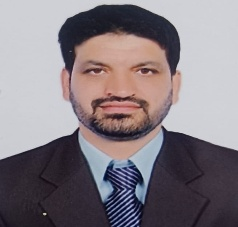
\includegraphics[width=2.2cm,height=2.7cm,keepaspectratio]{author1.jpg}
	\end{minipage}\hfill
	\begin{minipage}[t]{0.80\columnwidth}
		\vspace{0pt}
		\textbf{Dr. Aijaz Ahmad Magray} is an Assistant Professor in the Department of Mathematics at JB Institute of Engineering and Technology (JBIET), Hyderabad, India. He received his Ph.D. in Mathematics from Devi Ahilya Vishwavidyalaya, Indore, India. His research interests include mathematical modeling, linear algebra, numerical analysis, optimization, and artificial intelligence applications in mathematics.
	\end{minipage}
	\par\vspace{1.5em}
	
	\noindent
	\begin{minipage}[t]{0.17\columnwidth}
		\vspace{0pt}
		\centering
		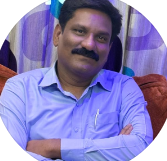
\includegraphics[width=2.2cm,height=2.7cm,keepaspectratio]{author2.png}
	\end{minipage}\hfill
	\begin{minipage}[t]{0.80\columnwidth}
		\vspace{5pt}
		\textbf{D. Raju} is an Assistant Professor in the Department of Mathematics, Jawaharlal Nehru Technological University, Hyderabad, India. His research focuses on applied mathematics, operations research, optimization, and mathematical modelling.
	\end{minipage}
	\par\vspace{1.5em}
	
	\noindent
	\begin{minipage}[t]{0.17\columnwidth}
		\vspace{0pt}
		\centering
		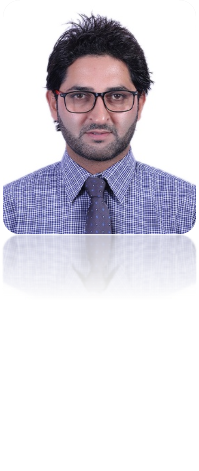
\includegraphics[width=5.2cm,height=5cm,keepaspectratio]{author3.png}
	\end{minipage}\hfill
	\begin{minipage}[t]{0.80\columnwidth}
		\vspace{5pt}
		\textbf{Dr. Aafaq A. Rather} is an Assistant Professor at the Symbiosis Statistical Institute, Symbiosis International (Deemed University), Pune, India. His research interests include probability distributions, statistical quality control, sampling theory, reliability analysis, and machine learning. He has published over 130 research papers in reputed international journals.
	\end{minipage}
	\par\vspace{-.5em}
	
	\noindent
	\begin{minipage}[t]{0.17\columnwidth}
		\vspace{0pt}
		\centering
		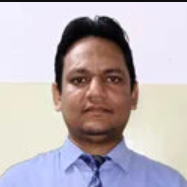
\includegraphics[width=2.2cm,height=2.7cm,keepaspectratio]{author4.png}
	\end{minipage}\hfill
	\begin{minipage}[t]{0.80\columnwidth}
		\vspace{0pt}
		\textbf{Dr. Ikram Ali} is an Assistant Professor in the Department of Computer Science and Engineering at Apex Institute of Technology, Chandigarh University, Punjab, India. His research interests include artificial intelligence, machine learning, data analytics, and computational intelligence.
	\end{minipage}
	\par\vspace{1.5em}
	
	\noindent
	\begin{minipage}[t]{0.17\columnwidth}
		\vspace{0pt}
		\centering
		
\includegraphics[width=2.2cm,height=2.7cm,keepaspectratio]{author5.jpg}
	\end{minipage}\hfill
	\begin{minipage}[t]{0.80\columnwidth}
		\vspace{0pt}
		\textbf{Dr. Vidya Yerneni} is associated with the Symbiosis Statistical Institute, Symbiosis International (Deemed University), Pune, India. Her research interests include applied statistics, statistical modelling, data science, and multivariate analysis.
	\end{minipage}
	\par\vspace{1.5em}
	
	\noindent
	\begin{minipage}[t]{0.17\columnwidth}
		\vspace{0pt}
		\centering
		
\includegraphics[width=2.2cm,height=2.7cm,keepaspectratio]{author6.jpg}
	\end{minipage}\hfill
	\begin{minipage}[t]{0.80\columnwidth}
		\vspace{0pt}
		\textbf{Dr. Ahmed A. F. Osman} is affiliated with the Applied College, King Faisal University, Al-Ahsa, Saudi Arabia. His research interests include applied mathematics, optimization, numerical analysis, and interdisciplinary mathematical applications.
	\end{minipage}
	
	\noindent
	\begin{minipage}[t]{0.17\columnwidth}
		\vspace{0pt}
		\centering
		
\includegraphics[width=2.2cm,height=2.7cm,keepaspectratio]{author7.jpg}
	\end{minipage}\hfill
	\begin{minipage}[t]{0.80\columnwidth}
		\vspace{0pt}
		\textbf{Dr. Mohammed Ataelfadiel} is with the Applied College, King Faisal University, Al-Ahsa, Saudi Arabia. His research focuses on applied mathematics, mathematical modelling, optimization, and computational methods.
	\end{minipage}
	\par\vspace{1.5em}
	
	\noindent
	\begin{minipage}[t]{0.17\columnwidth}
		\vspace{0pt}
		\centering
		
\includegraphics[width=2.2cm,height=2.7cm,keepaspectratio]{author8.jpg}
	\end{minipage}\hfill
	\begin{minipage}[t]{0.80\columnwidth}
		\vspace{0pt}
		\textbf{Dr. Ala Abdullah} is a faculty member at the Applied College, King Faisal University, Al-Ahsa, Saudi Arabia. Her research interests include applied mathematics, statistics, mathematical modelling, and data analysis.
	\end{minipage}
	\par\vspace{1.5em}
	
	\noindent
	\begin{minipage}[t]{0.17\columnwidth}
		\vspace{0pt}
		\centering
		
\includegraphics[width=2.2cm,height=2.7cm,keepaspectratio]{author9.jpg}
	\end{minipage}\hfill
	\begin{minipage}[t]{0.80\columnwidth}
		\vspace{0pt}
		\textbf{Dr. Maryam Nasser Almusallam} is affiliated with the Applied College, King Faisal University, Al-Ahsa, Saudi Arabia. Her research interests include applied mathematics, statistical analysis, educational research, and computational methods.
	\end{minipage}
	\par\vspace{1.5em}
	
	\noindent
	\begin{minipage}[t]{0.17\columnwidth}
		\vspace{0pt}
		\centering
		
\includegraphics[width=2.2cm,height=2.7cm,keepaspectratio]{author10.jpg}
	\end{minipage}\hfill
	\begin{minipage}[t]{0.80\columnwidth}
		\vspace{0pt}
		\textbf{Dr. Osman Elwasila Elshiekh} is a faculty member in the Department of Management Information Systems, College of Business Administration, King Faisal University, Saudi Arabia. His research interests include management information systems, data analytics, artificial intelligence, and business intelligence.
	\end{minipage}
	\par\vspace{1.5em}
	
	\noindent
	\begin{minipage}[t]{0.17\columnwidth}
		\vspace{0pt}
		\centering
		
\includegraphics[width=2.2cm,height=2.7cm,keepaspectratio]{author11.jpg}
	\end{minipage}\hfill
	\begin{minipage}[t]{0.80\columnwidth}
		\vspace{0pt}
		\textbf{Dr. Ali Salem Bin Sama} is affiliated with the Department of Management Information Systems, College of Business Administration, King Faisal University, Saudi Arabia. His research interests include information systems, digital transformation, data analytics, and decision support systems.
	\end{minipage}
	\par\vspace{1.5em}
	
	\noindent
	\begin{minipage}[t]{0.17\columnwidth}
		\vspace{0pt}
		\centering
		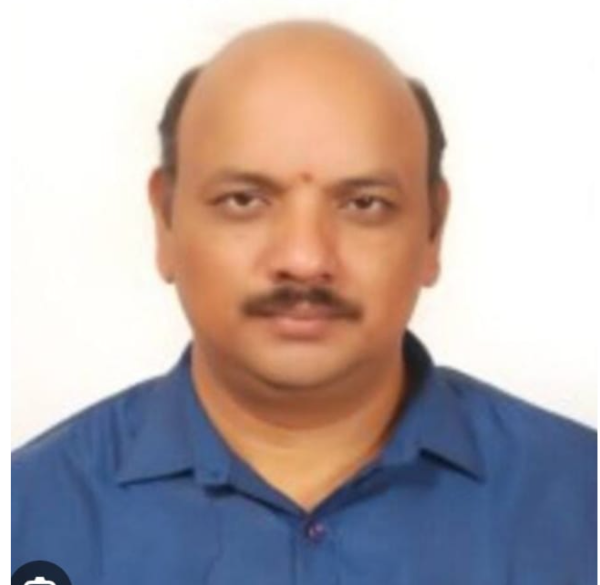
\includegraphics[width=2.2cm,height=2.7cm,keepaspectratio]{author12.png}
	\end{minipage}\hfill
	\begin{minipage}[t]{0.80\columnwidth}
		\vspace{0pt}
		\textbf{Dr. P. Srinivasa Rao} is a Professor in the Department of Computer Science and Engineering at JB Institute of Engineering and Technology (JBIET), Hyderabad. He received his Ph.D. from Jawaharlal Nehru Technological University Hyderabad (JNTUH). His research interests include cloud computing, distributed systems, data science, and database management systems.
	\end{minipage}
	
\end{document}
